\documentclass[a4paper, 11pt]{article}
\usepackage{graphicx}
\graphicspath{{../figures/}}

\usepackage{amsmath}
\usepackage{amssymb}
\usepackage{adjustbox}
\usepackage{multirow}

\begin{document}

\section{Supplementary Materials}

\renewcommand{\thefigure}{S\arabic{figure}}
\setcounter{figure}{0}
\renewcommand{\thetable}{S\arabic{table}}
\setcounter{table}{0}

\subsection{Pre-processing}

\begin{figure}[!h]
\centerline{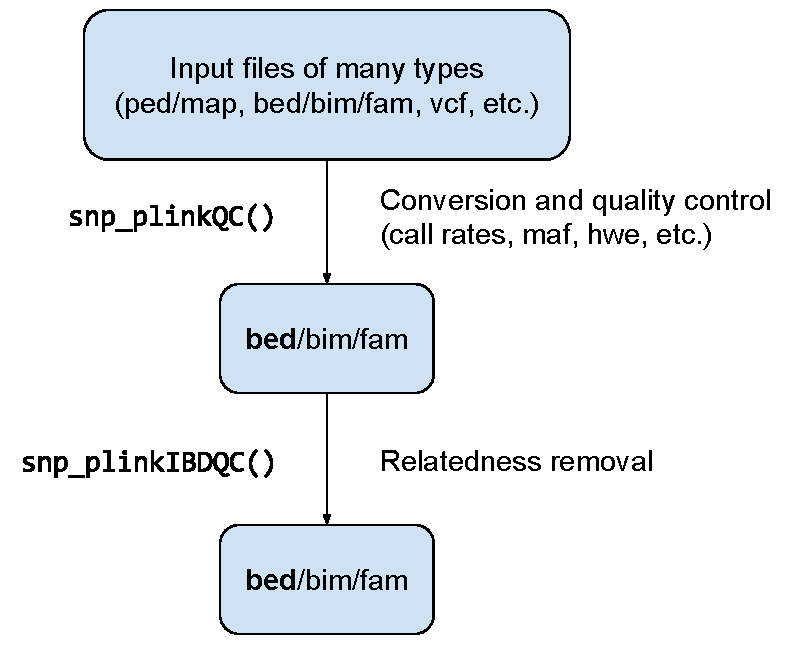
\includegraphics[width=\linewidth]{conversion-QC.pdf}}
\caption{Conversion and quality control preprocessing functions available in package bigsnpr via system calls to PLINK.}\label{fig:qc}
\end{figure}

\clearpage

\begin{figure}[!h]
\centerline{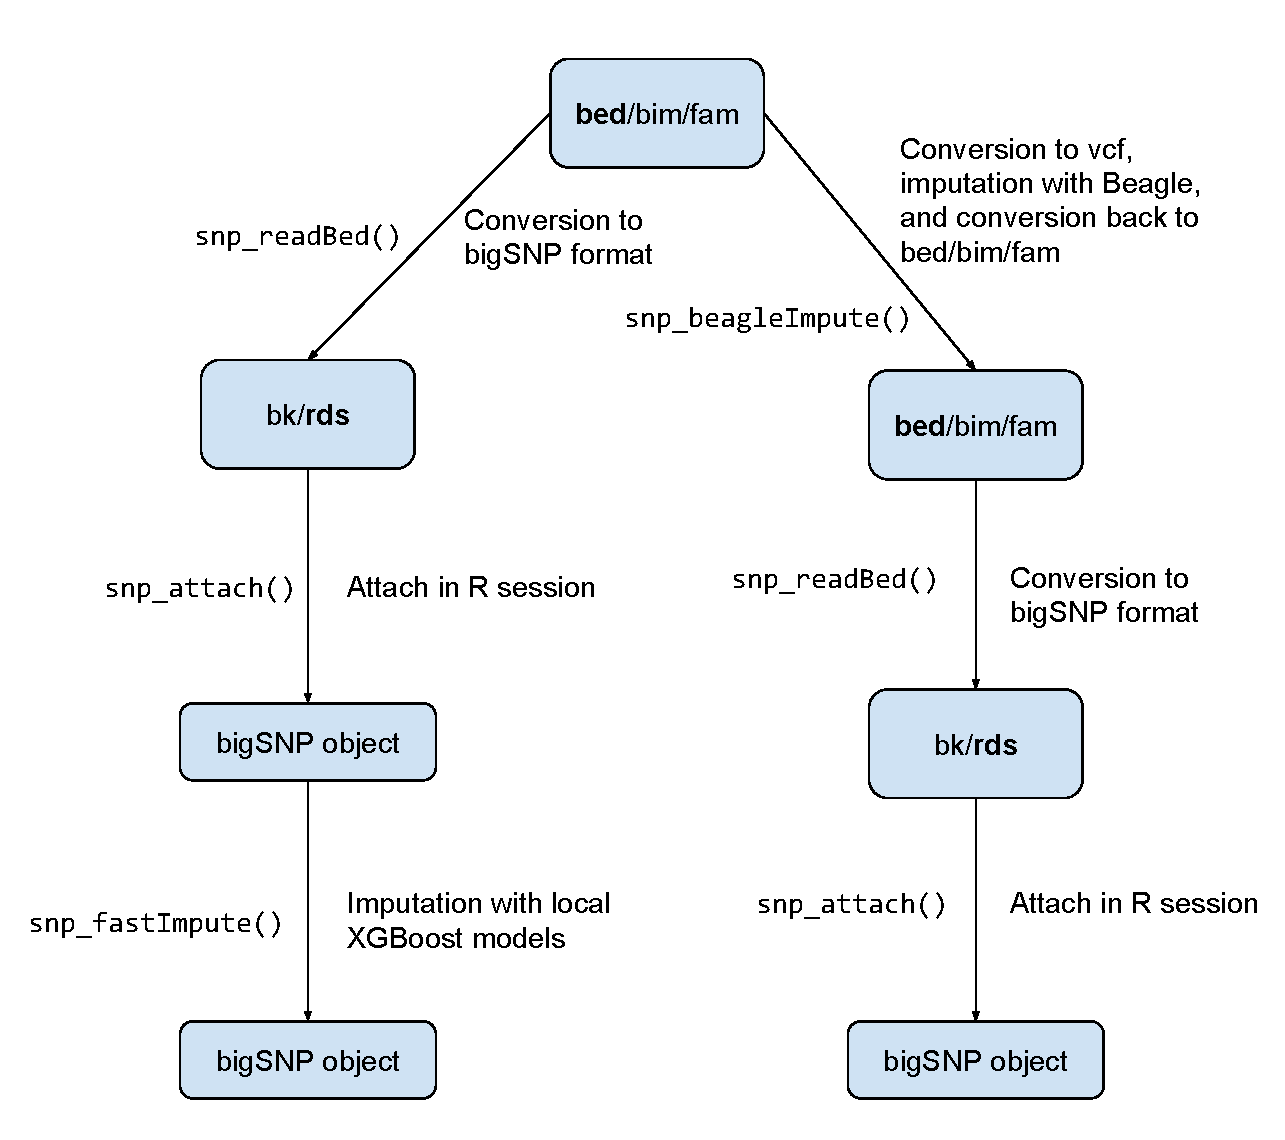
\includegraphics[width=\linewidth]{imputation.pdf}}
\caption{Imputation and reading functions available in package bigsnpr.}\label{fig:impute}
\end{figure}

\clearpage

\subsection{Long-range LD regions}

\begin{table}[!h]
\centering
\begin{tabular}{lccc}
  \hline
 & Chromosome & Start (Mb) & Stop (Mb) \\ 
  \hline
1 &  2 & 134.7 (134.5) & 137.3 (138) \\ 
  2 &  6 & 27.5 (25.5) & 33.1 (33.5) \\ 
  3 &  8 & 6.6 (8) & 13.2 (12) \\ 
   \hline
\end{tabular}
\caption{\label{tab:lrldr-popres}Regions found by snp\_autoSVD for the POPRES dataset. Numbers in parentheses correspond to regions referenced in Price et al., 2008.}
\end{table}

\vspace{5em}

% latex table generated in R 3.3.3 by xtable 1.8-2 package
% Tue Jun 13 11:29:13 2017
\begin{table}[!h]
\centering
\begin{tabular}{l|cccccccccc}
  \hline
 & PC1 & PC2 & PC3 & PC4 & PC5 & PC6 & PC7 & PC8 & PC9 & PC10 \\
  \hline
PC1 & 100.0 & -0.1 & -0.0 & 0.1 & -0.1 & 0.0 & 0.0 & 0.0 & -0.0 & -0.0 \\
  PC2 & 0.1 & 100.0 & -0.0 & 0.1 & -0.0 & -0.0 & -0.0 & 0.2 & -0.1 & -0.0 \\
  PC3 & 0.0 & -0.0 & 99.9 & 0.9 & 0.1 & -0.1 & -0.3 & 0.2 & 0.4 & 0.1 \\
  PC4 & -0.1 & -0.1 & -0.9 & 99.7 & -1.0 & 0.7 & 0.6 & 0.2 & 0.3 & 0.9 \\
  PC5 & 0.1 & 0.0 & -0.1 & 1.1 & 99.3 & 1.3 & -0.8 & 1.3 & -4.2 & -2.4 \\
  PC6 & -0.0 & 0.0 & 0.1 & -0.7 & -1.0 & 97.7 & -3.5 & 6.1 & 7.9 & -6.2 \\
  PC7 & -0.0 & -0.1 & 0.2 & -0.3 & -1.7 & 0.3 & 58.3 & 73.2 & -25.9 & 9.1 \\
  PC8 & 0.1 & -0.1 & -0.3 & 0.4 & -0.5 & -5.3 & -73.5 & 59.5 & 15.8 & 13.2 \\
  PC9 & 0.0 & 0.1 & -0.4 & -0.8 & 5.0 & -7.6 & 27.8 & 11.0 & 91.9 & 9.0 \\
  PC10 & 0.1 & 0.0 & 0.0 & -0.9 & 1.6 & 10.2 & 3.9 & -19.6 & -6.3 & 89.2 \\
   \hline
\end{tabular}
\caption{Correlation between scores of PCA for the POPRES dataset  when automatically removing long-range LD regions and when removing them based on a predefined table.}
\label{tab:pc-popres}
\end{table}

\clearpage

% latex table generated in R 3.3.3 by xtable 1.8-2 package
% Tue Jul 18 15:59:51 2017
\begin{table}[!h]
\centering
\begin{tabular}{lccc}
  \hline
 & Chromosome & Start (Mb) & Stop (Mb) \\ 
  \hline
1 &  2 & 134.4 (134.5) & 138.1 (138) \\ 
  2 &  6 & 23.8 (25.5) & 35.8 (33.5) \\ 
  3 &  8 & 6.3 (8) & 13.5 (12) \\ 
  4 &  3 & 163.1 (n/a) & 164.9 (n/a) \\ 
  5 & 14 & 46.6 (n/a) & 47.5 (n/a) \\ 
   \hline
\end{tabular}
\caption{Regions found by snp\_autoSVD for the celiac dataset. Numbers in parentheses correspond to regions referenced in Price et al., 2008.}
\label{tab:lrldr-celiac}
\end{table}

\vspace{5em}

% latex table generated in R 3.3.3 by xtable 1.8-2 package
% Tue Jun 13 11:25:56 2017
\begin{table}[!h]
\centering
\begin{tabular}{l|cccccccccc}
  \hline
 & PC1 & PC2 & PC3 & PC4 & PC5 & PC6 & PC7 & PC8 & PC9 & PC10 \\
  \hline
PC1 & 100.0 & -0.1 & -0.1 & 0.0 & 0.0 & 0.0 & 0.0 & 0.0 & 0.0 & 0.0 \\
  PC2 & 0.1 & 100.0 & 0.0 & 0.0 & -0.0 & -0.0 & 0.0 & -0.0 & -0.0 & -0.0 \\
  PC3 & 0.1 & -0.0 & 99.9 & 0.2 & -0.0 & 0.1 & 0.1 & 0.1 & 0.0 & -0.1 \\
  PC4 & -0.0 & -0.0 & -0.3 & 99.9 & -0.1 & 0.1 & -0.1 & 0.0 & 0.1 & 0.1 \\
  PC5 & 0.0 & 0.0 & 0.0 & 0.1 & 99.7 & 0.9 & -0.3 & 0.1 & -0.8 & -0.6 \\
  PC6 & -0.0 & 0.0 & -0.1 & -0.2 & -0.8 & 99.6 & 0.5 & -0.5 & -0.2 & -0.4 \\
  PC7 & -0.0 & 0.0 & -0.1 & 0.0 & 0.5 & -0.4 & 98.9 & 3.1 & 0.7 & 1.6 \\
  PC8 & 0.0 & 0.0 & -0.2 & -0.0 & -0.2 & 0.5 & -3.2 & 98.4 & -4.5 & -1.5 \\
  PC9 & -0.0 & -0.0 & -0.0 & 0.0 & 0.6 & 0.1 & -0.7 & 4.6 & 96.9 & -10.7 \\
  PC10 & -0.0 & -0.0 & 0.1 & -0.1 & 0.3 & 0.1 & -1.2 & 1.5 & 8.6 & 92.7 \\
   \hline
\end{tabular}
\caption{Correlation between scores of PCA for the Celiac dataset  when automatically removing long-range LD regions and when removing them based on a predefined table.}
\label{tab:pc-celiac}
\end{table}

\clearpage

\begin{figure}[!h]
\centerline{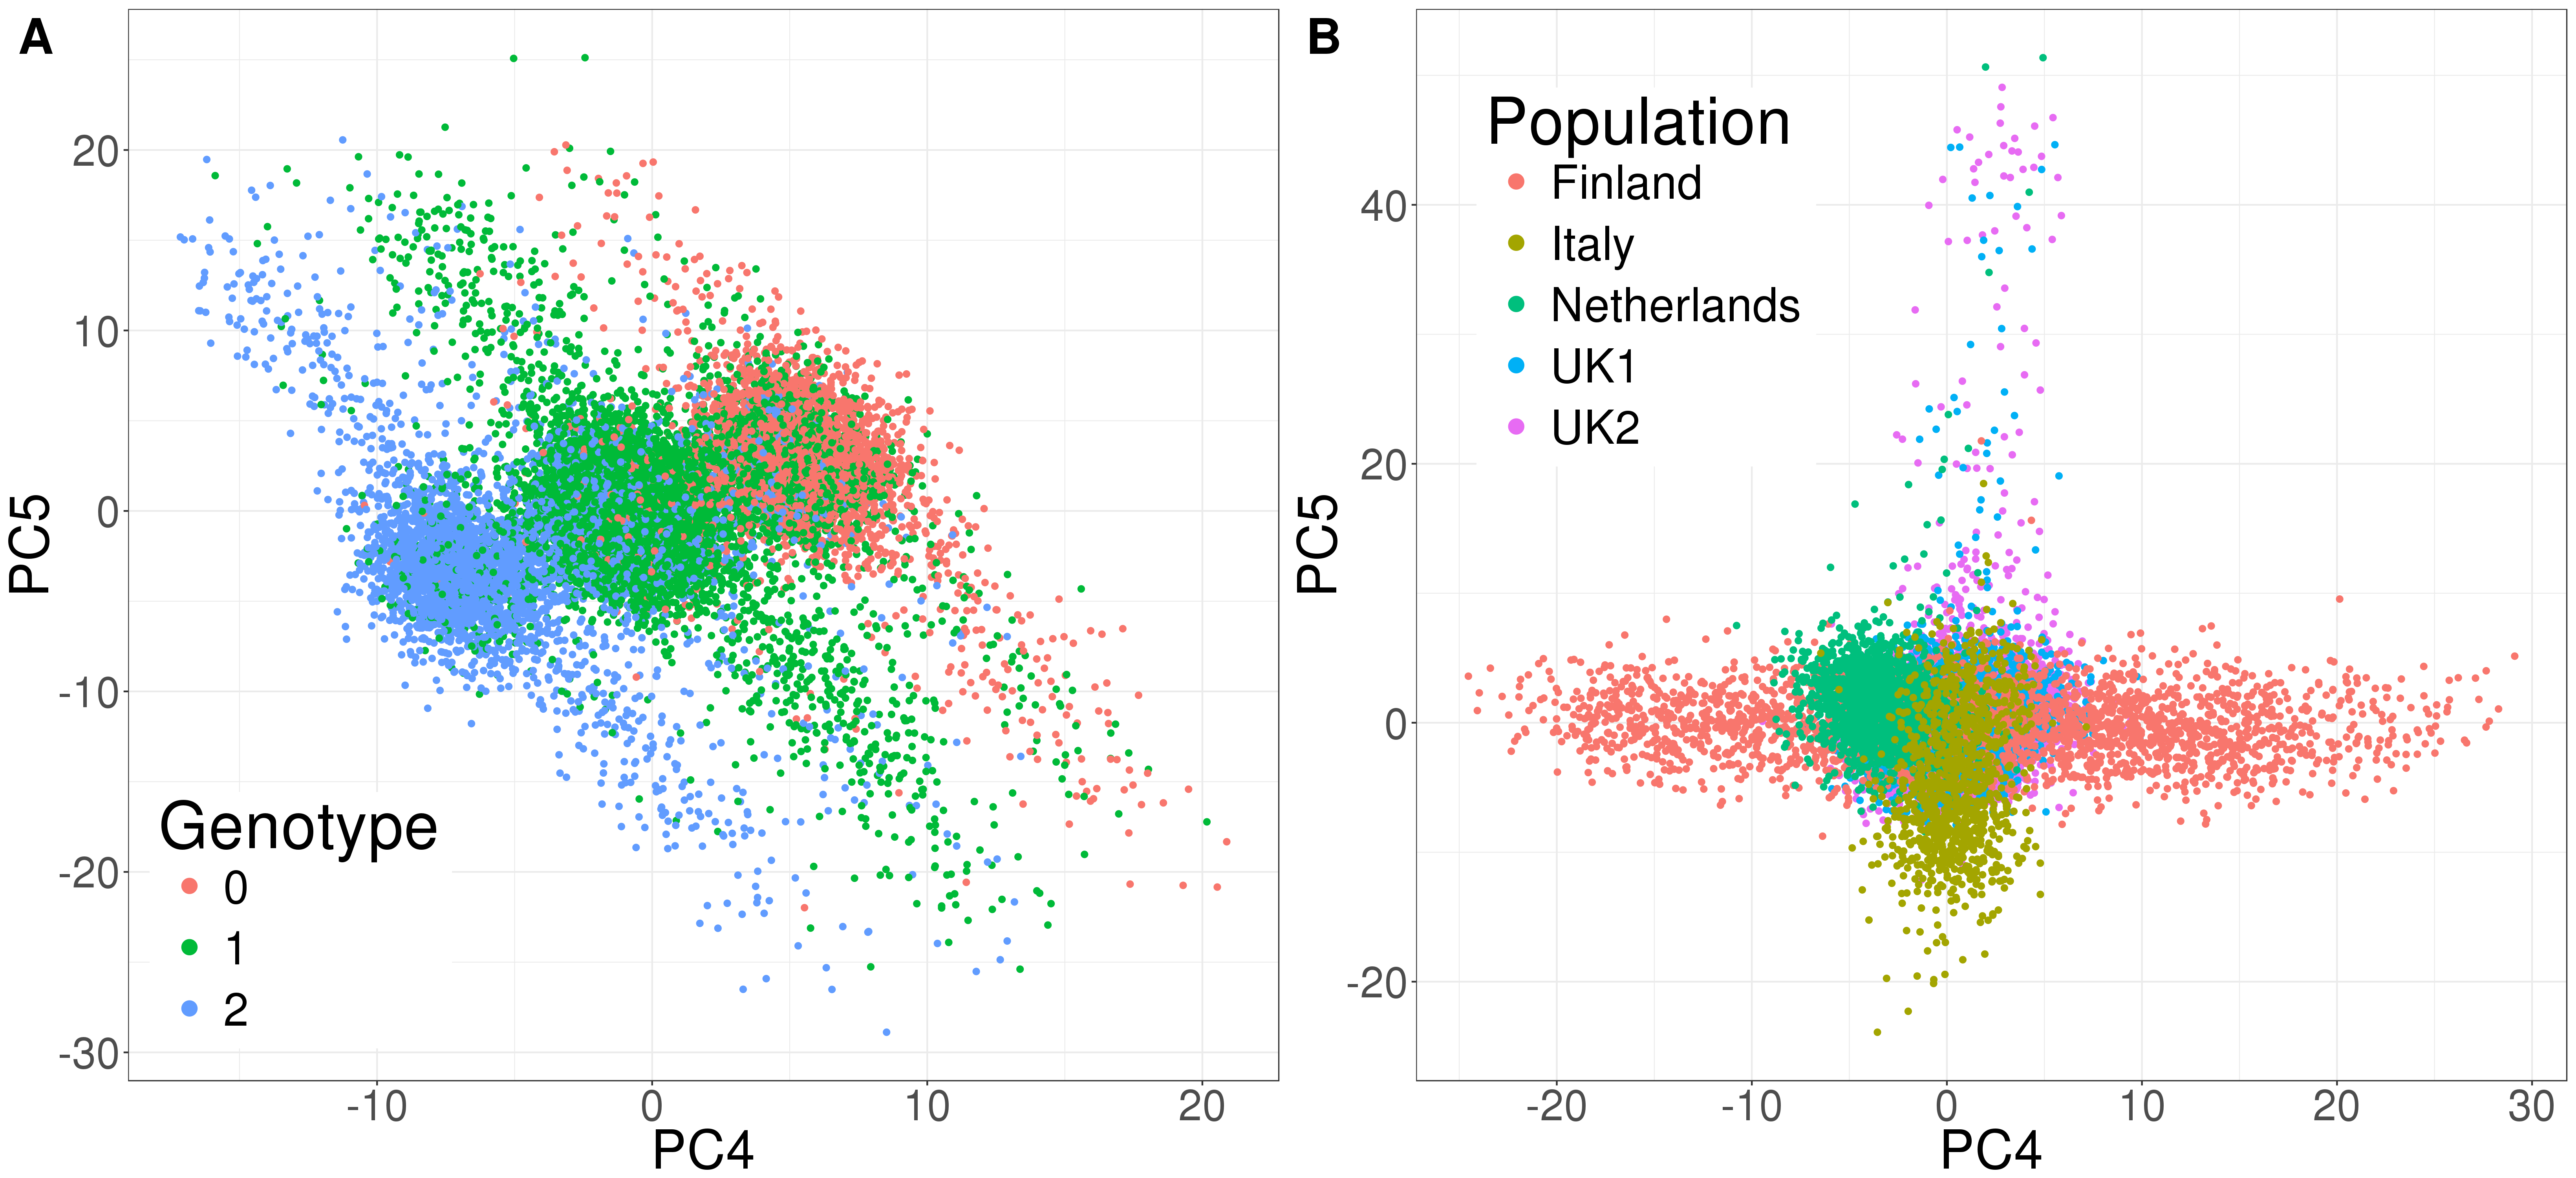
\includegraphics[width=\textwidth]{scores}}
\caption{PC4 and PC5 of the celiac disease dataset. Left panel, PC scores obtained without removing any long range LD region (only clumping at $r^2 > 0.2$). Individuals are coloured according to their genotype at the SNP that has the highest loading for PC4. Right panel, PC scores obtained with the automatic detection and removal of long-range LD regions. Individuals are coloured according to their population of origin.}\label{fig:scores}
\end{figure}

\vspace{3em}

\begin{figure}[!h]
\centerline{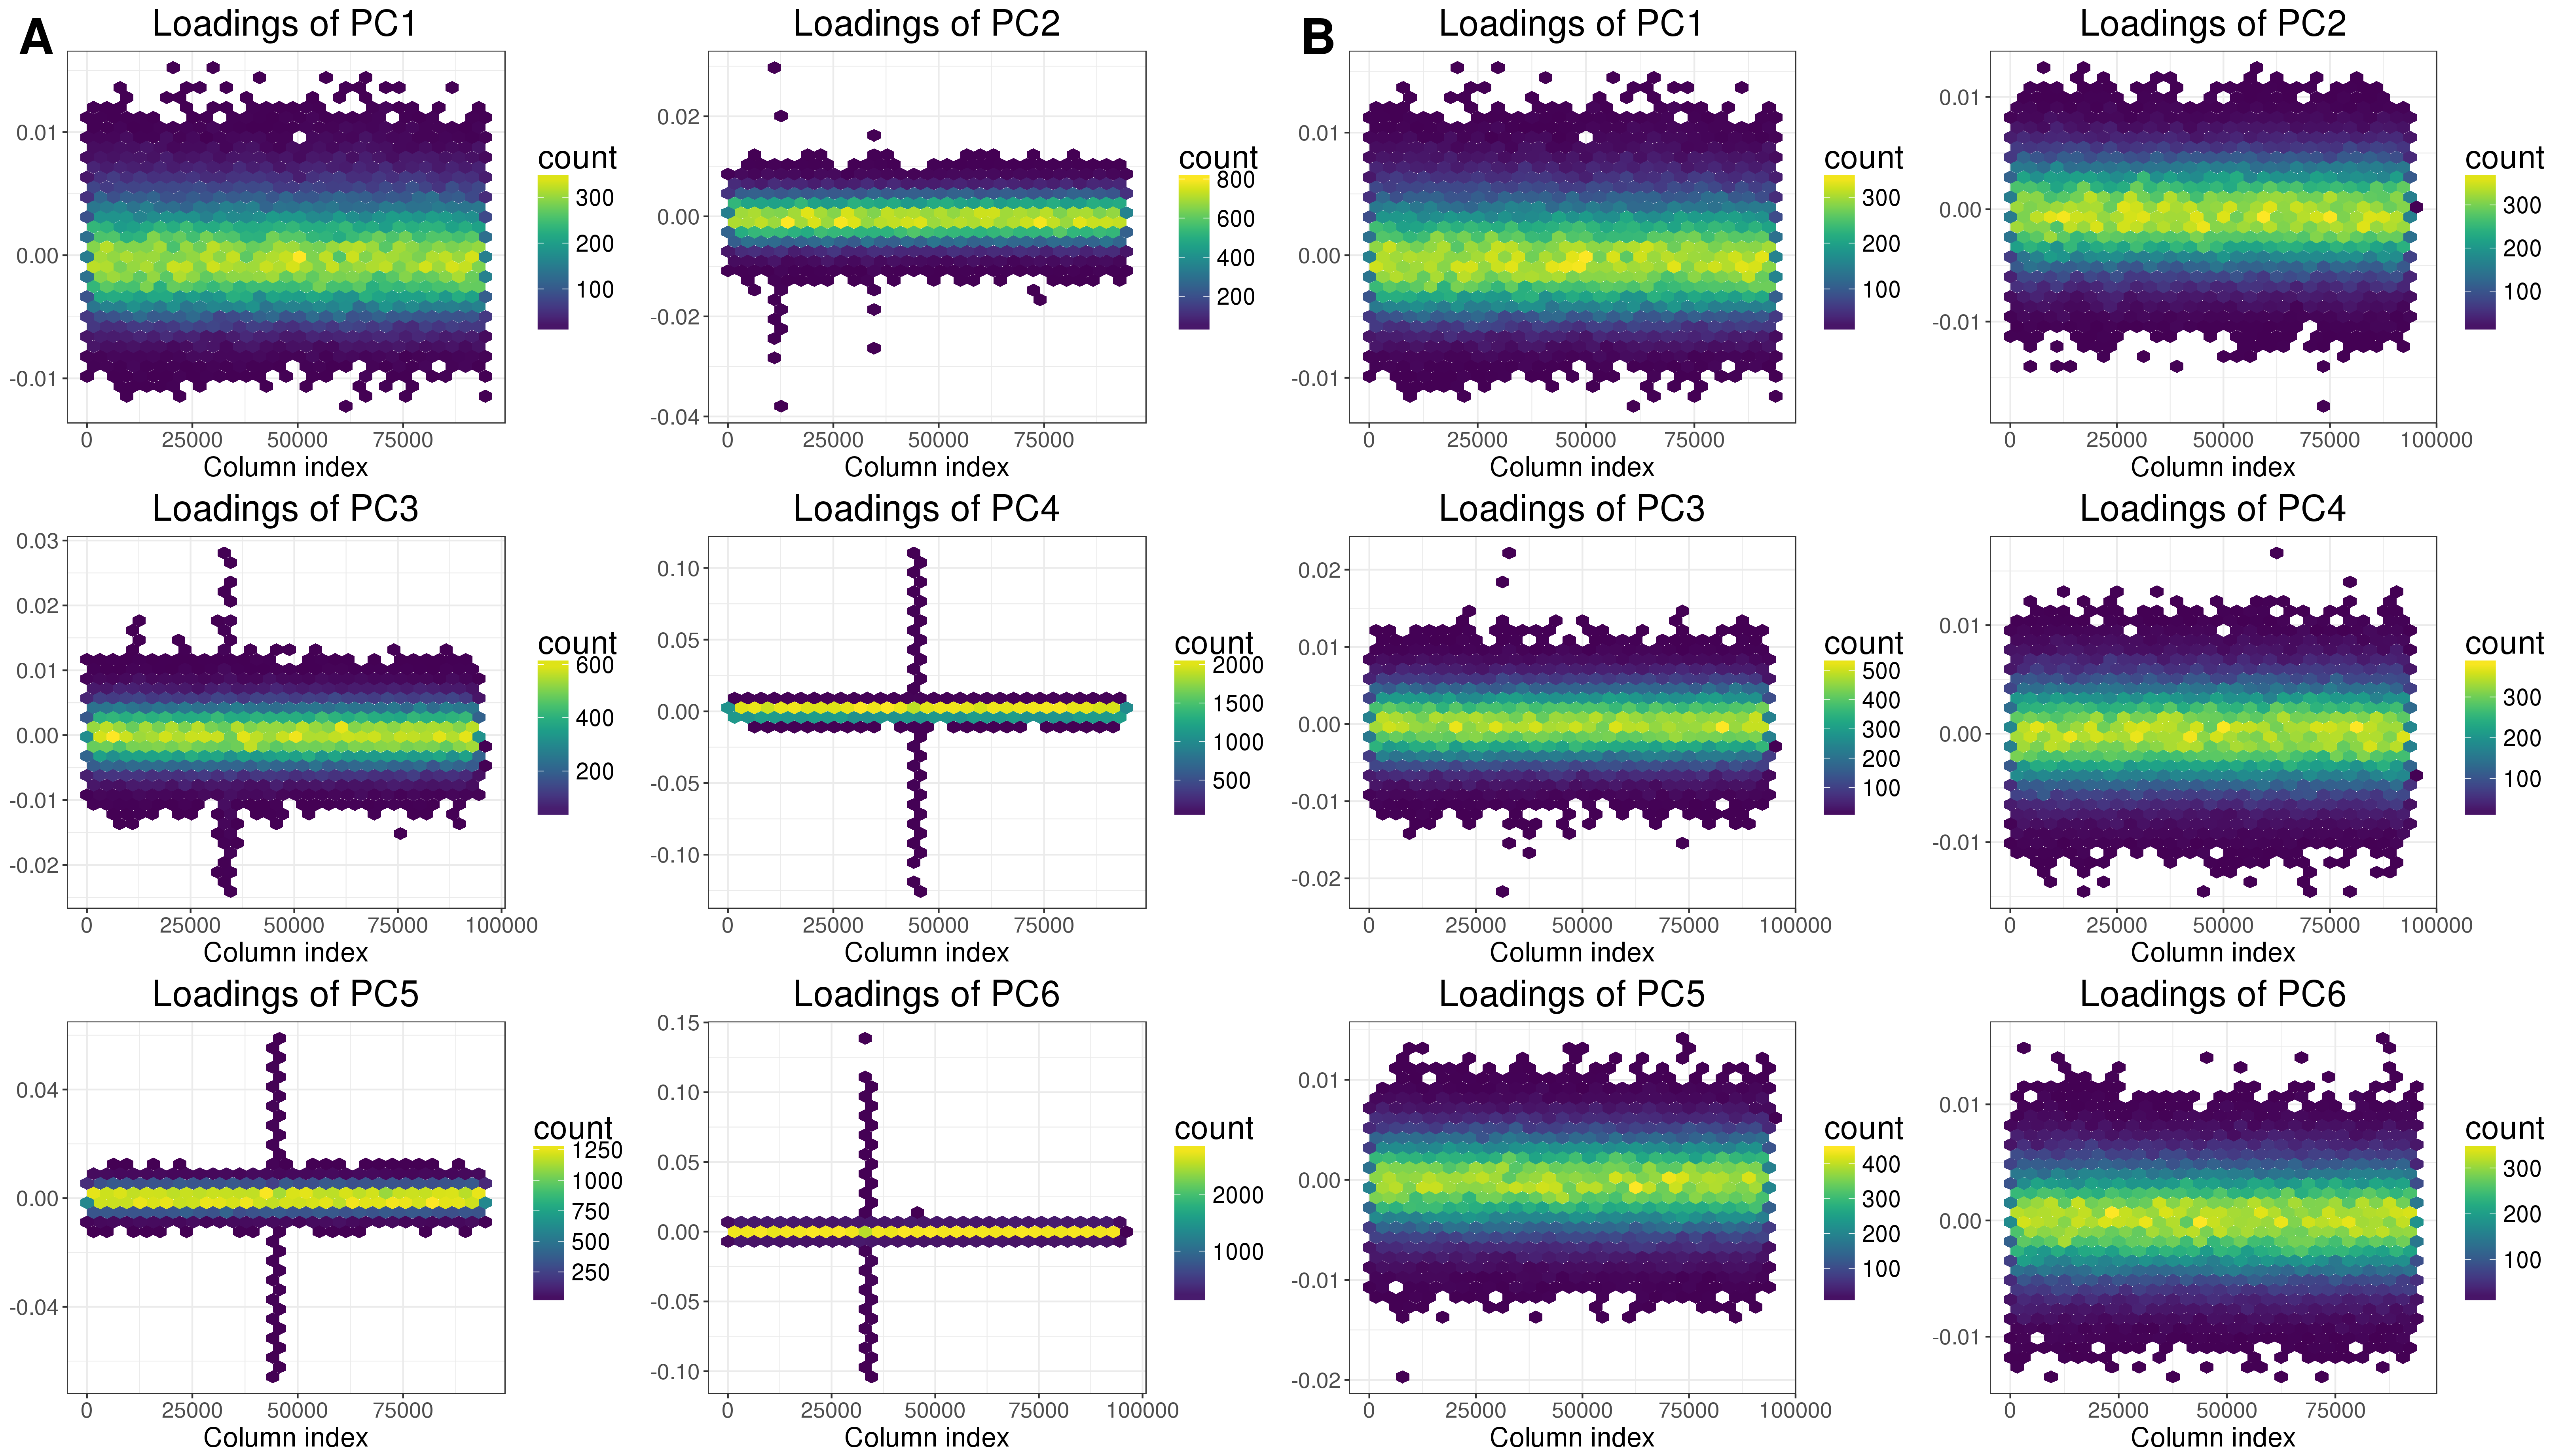
\includegraphics[width=\textwidth]{loadings}}
\caption{Loadings of first 6 PCs of the celiac disease dataset plotted as hexbins (2-D histogram with hexagonal cells). On the left, without removing any long range LD region (only clumping at $r^2 > 0.2$). On the right, with the automatic detection and removal of long-range LD regions.}\label{fig:loadings}
\end{figure}

\vspace{3em}

\begin{figure}[!h]
\centerline{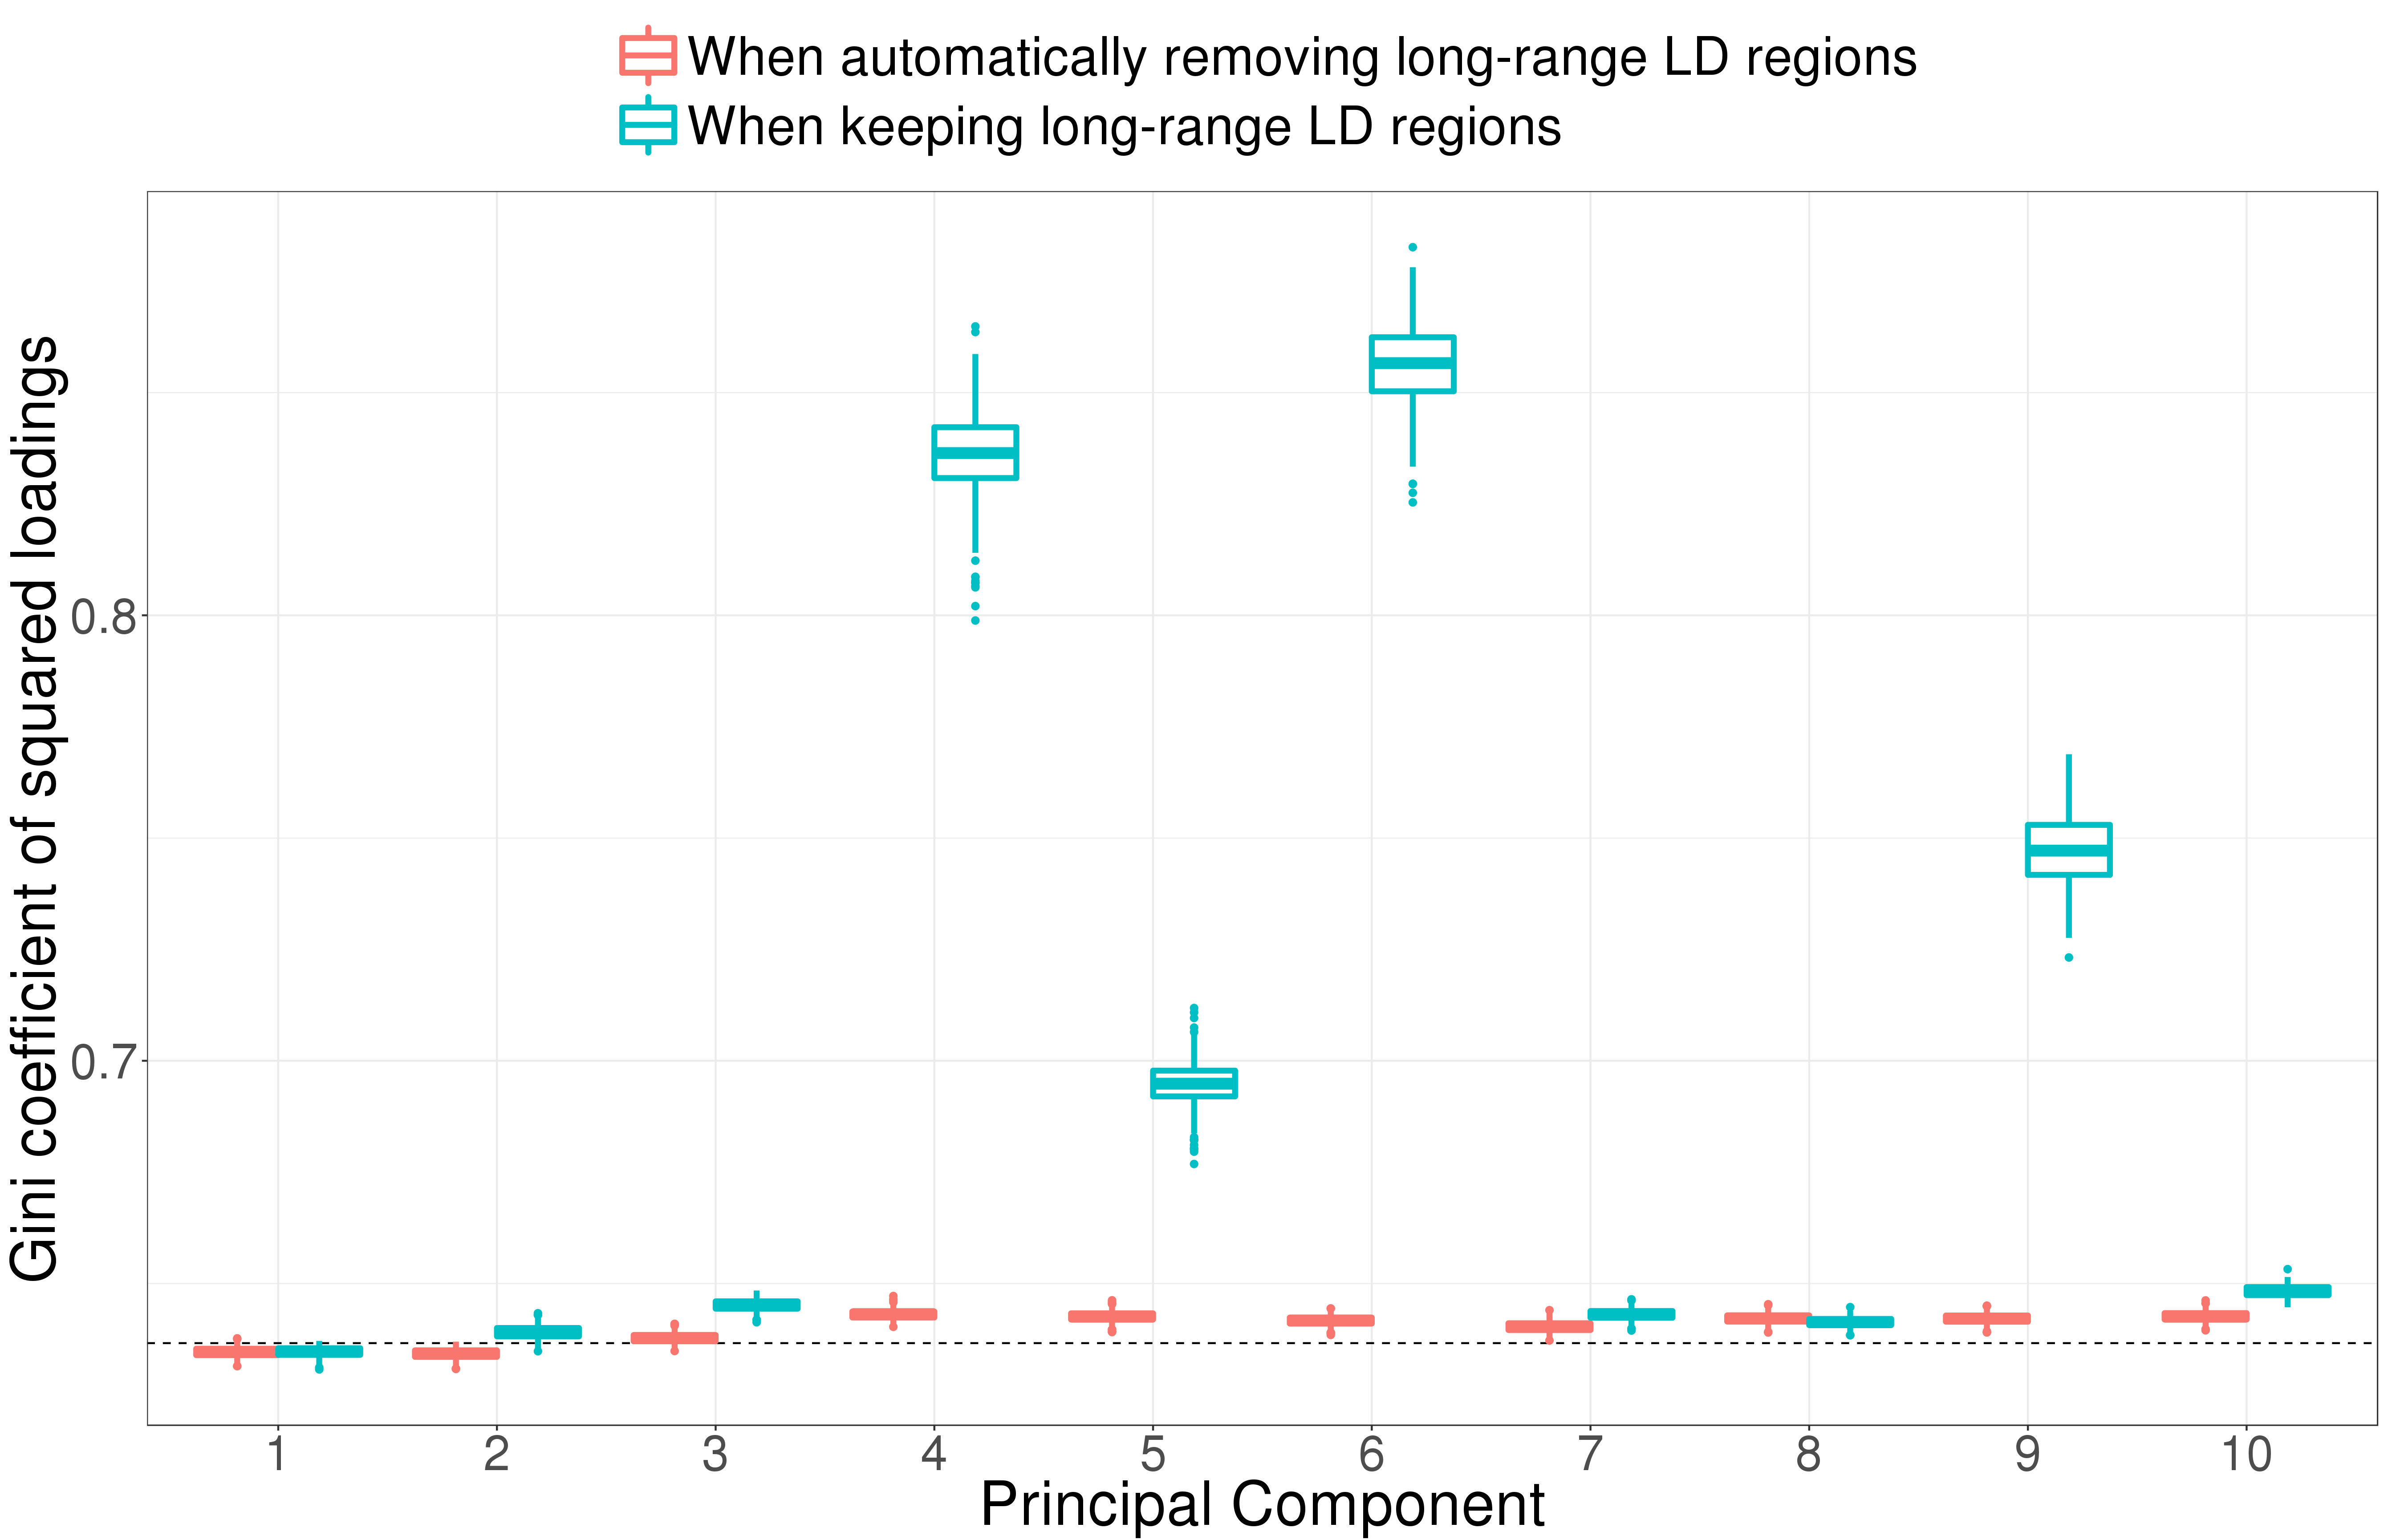
\includegraphics[width=\textwidth]{gini}}
\caption{Boxplots of 1000 bootstrapped Gini coefficients (measure of statistical dispersion) of squared loadings without removing any long range LD region (only clumping at $r^2 > 0.2$) and with the automatic detection and removal of long-range LD regions. The dashed line corresponds to the theoretical value for gaussian loadings.}\label{fig:gini}
\end{figure}

\clearpage

\subsection{Imputation}

\begin{figure}[!h]
\centerline{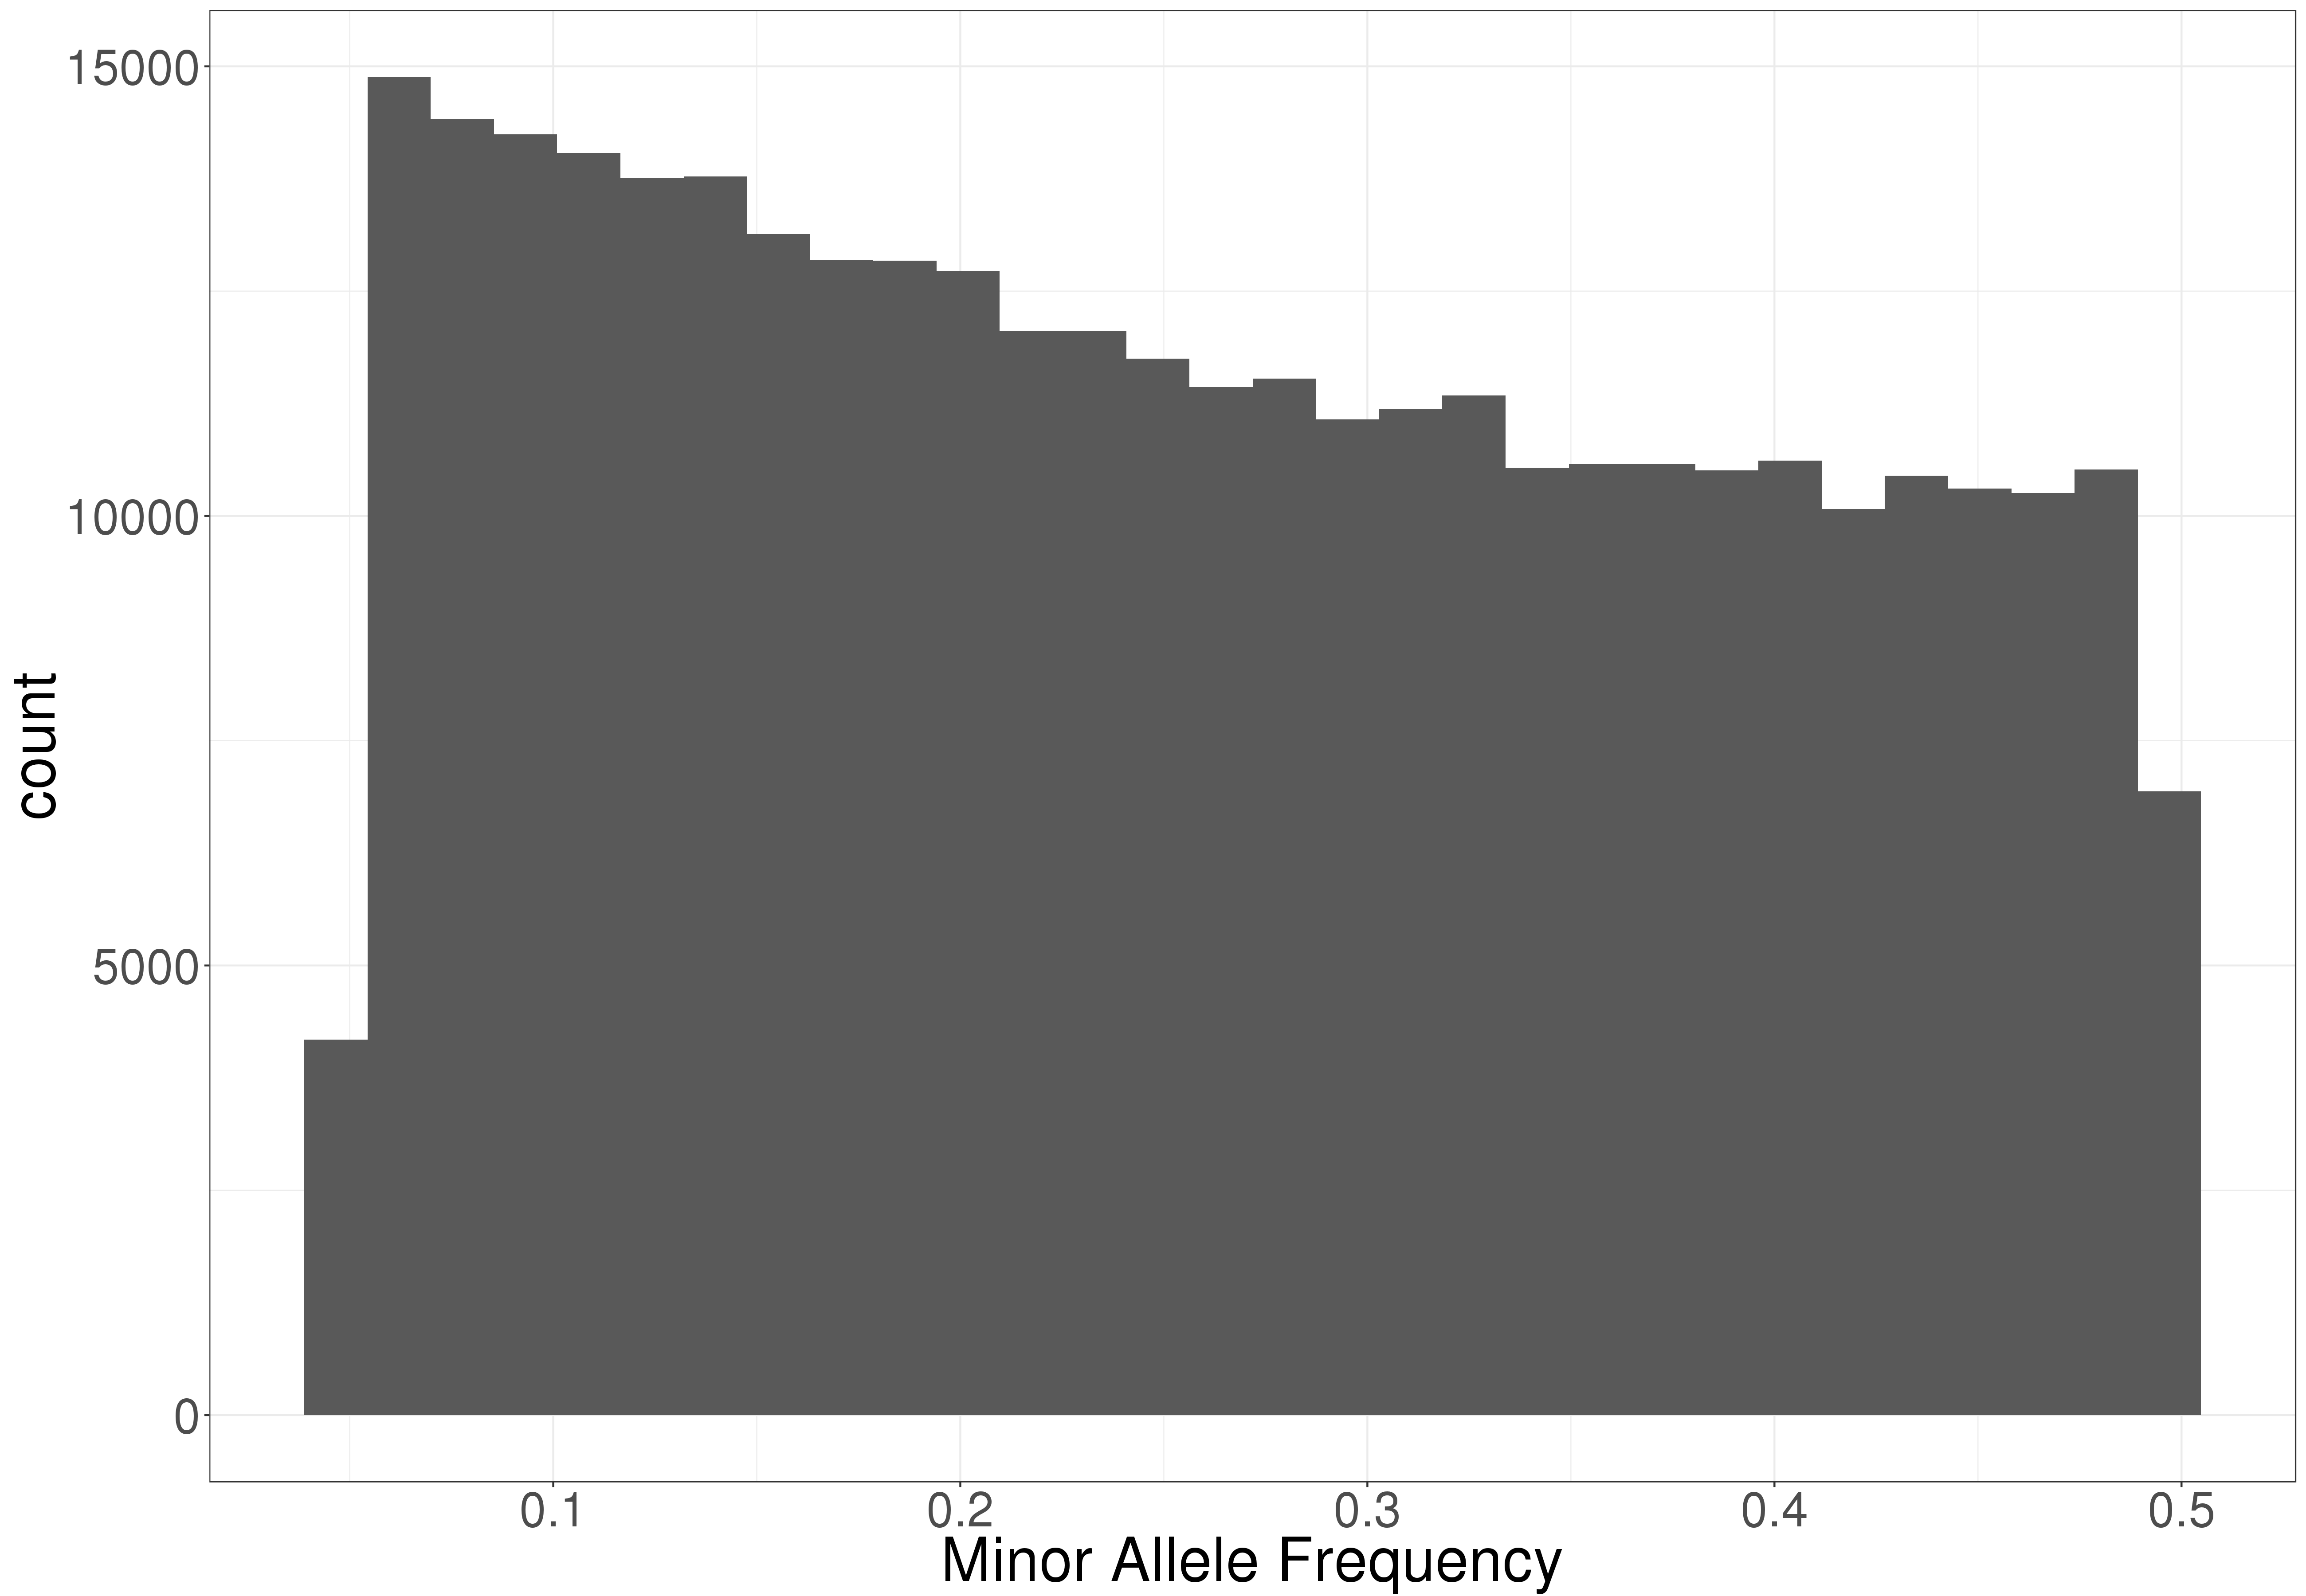
\includegraphics[width=\textwidth]{hist-maf}}
\caption{Histogram of the minor allele frequencies of the POPRES dataset used for comparing imputation methods.}\label{fig:maf}
\end{figure}

\vspace{3em}

\begin{figure}[!h]
\centerline{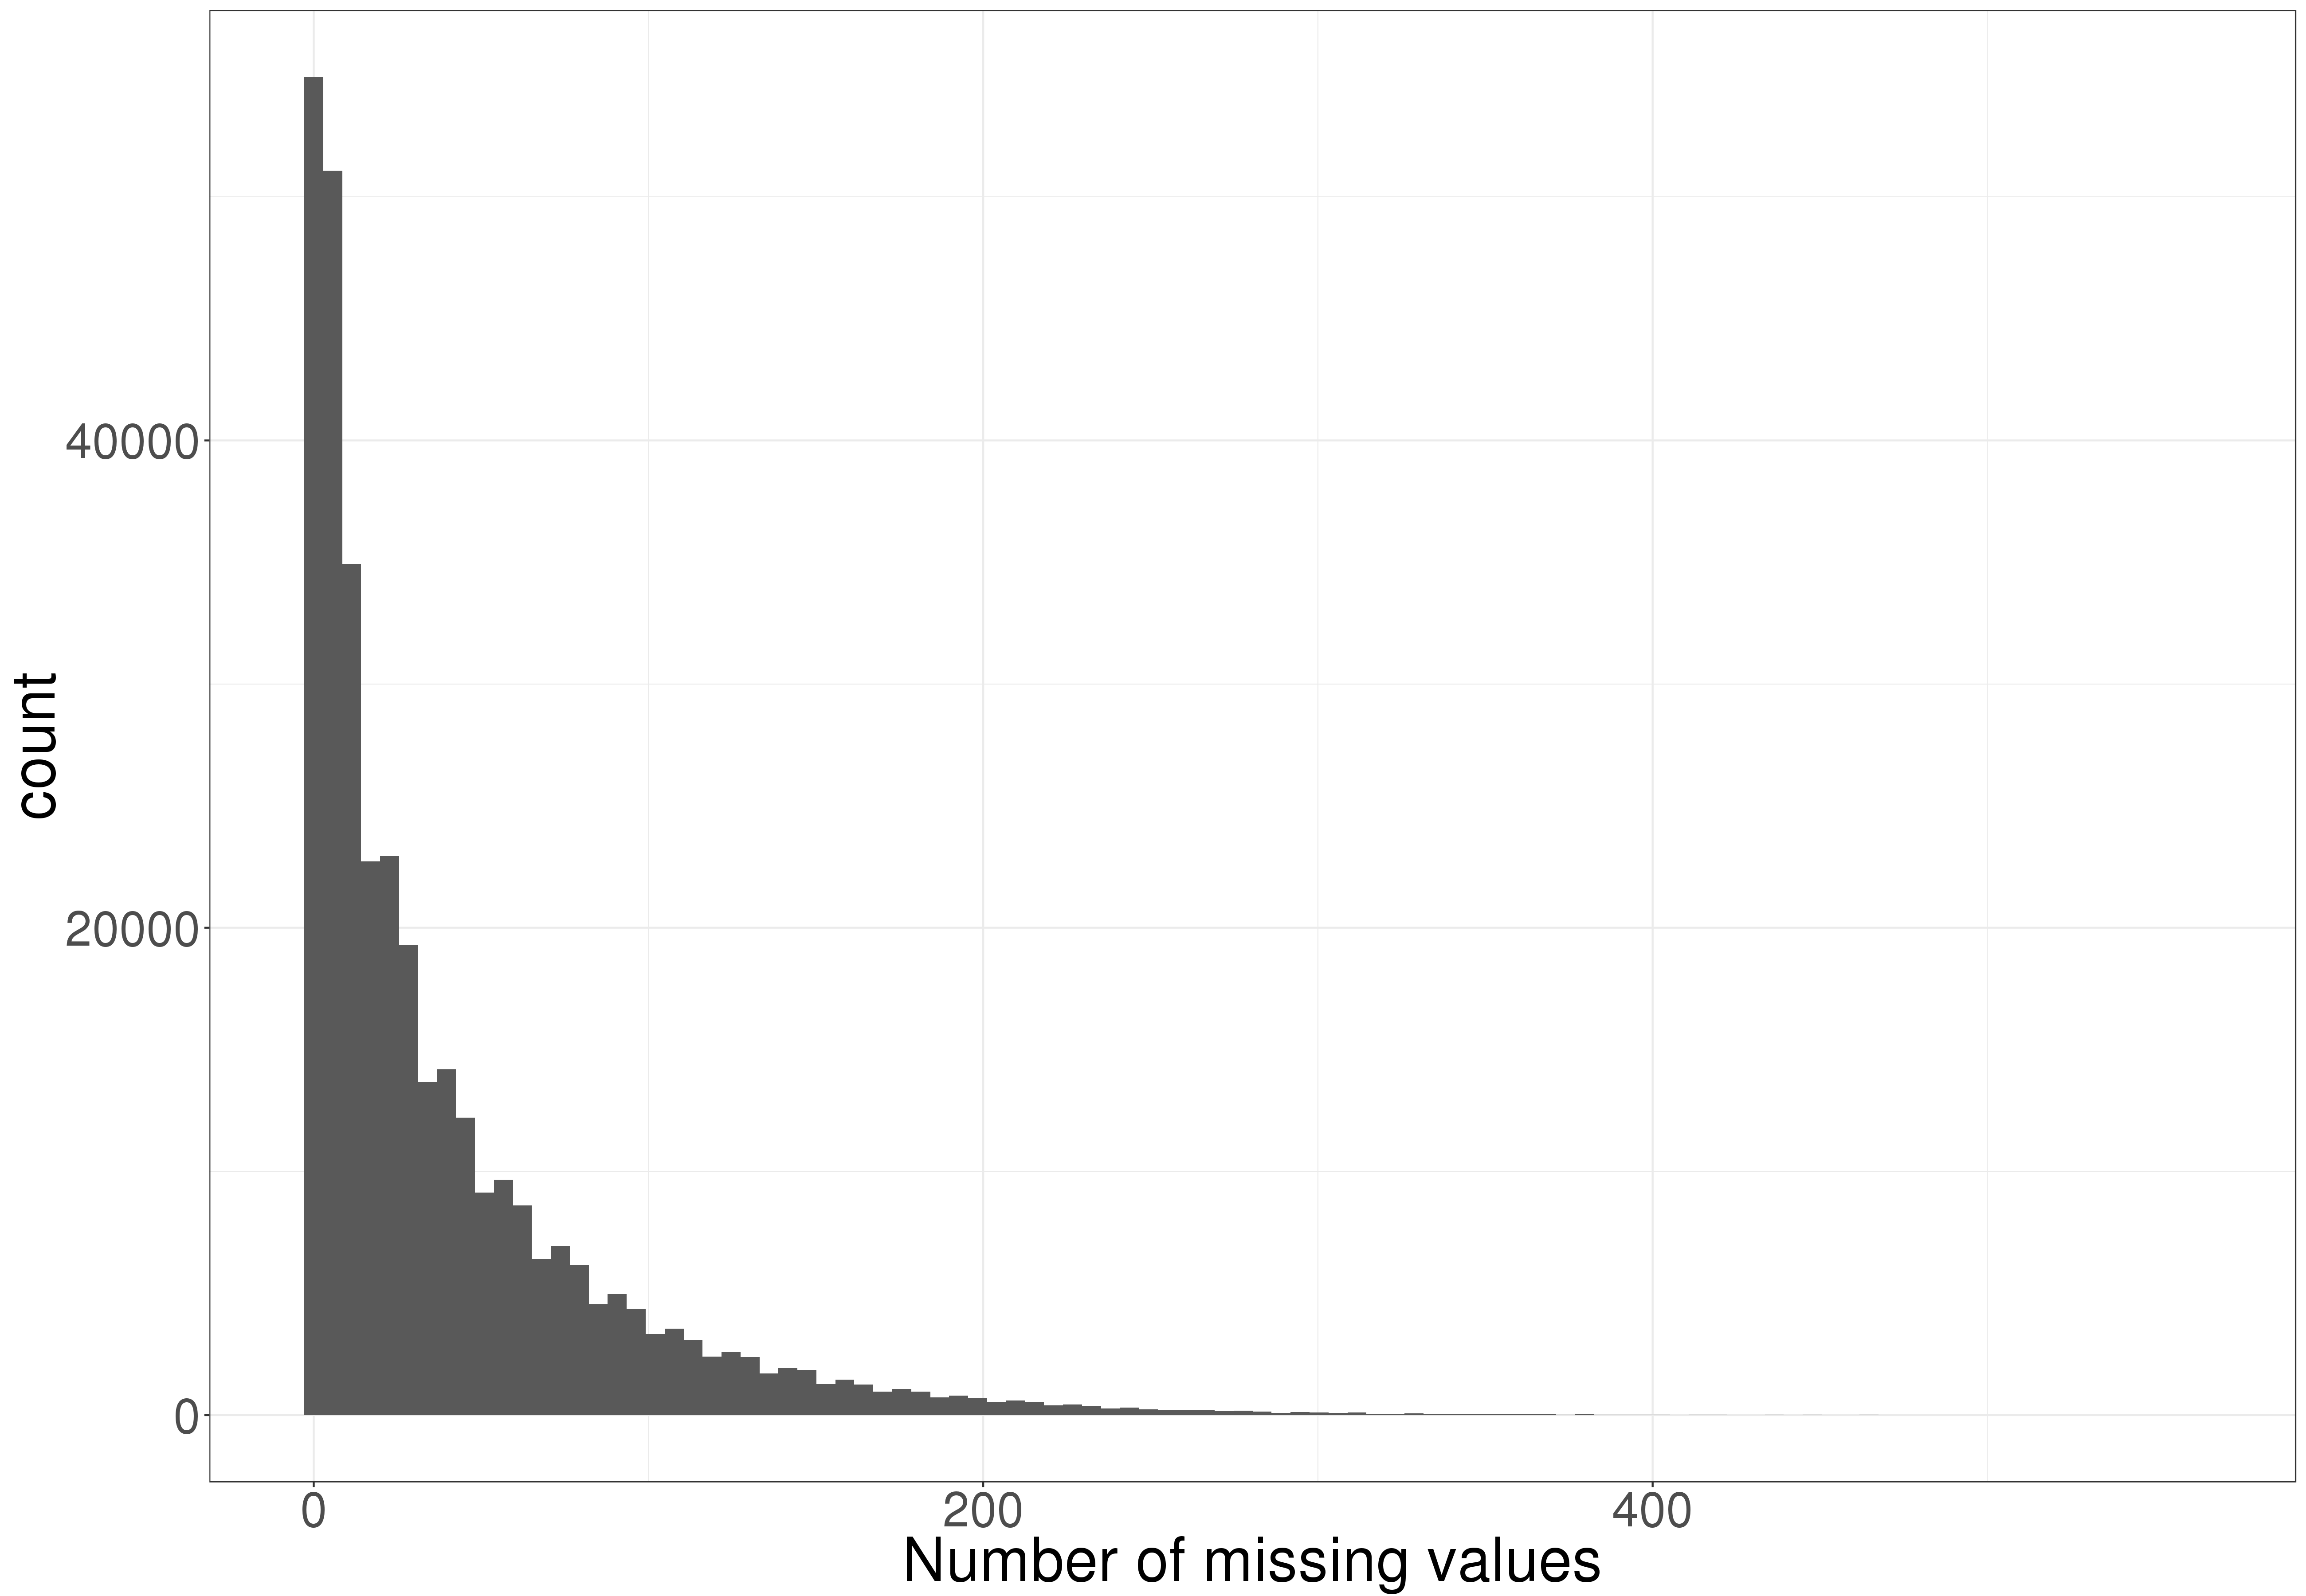
\includegraphics[width=\textwidth]{hist-NA}}
\caption{Histogram of the number of missing values by SNP. These numbers were generated using a Beta-binomial distribution.}\label{fig:NA}
\end{figure}

\vspace{3em}

\begin{figure}[!h]
\centerline{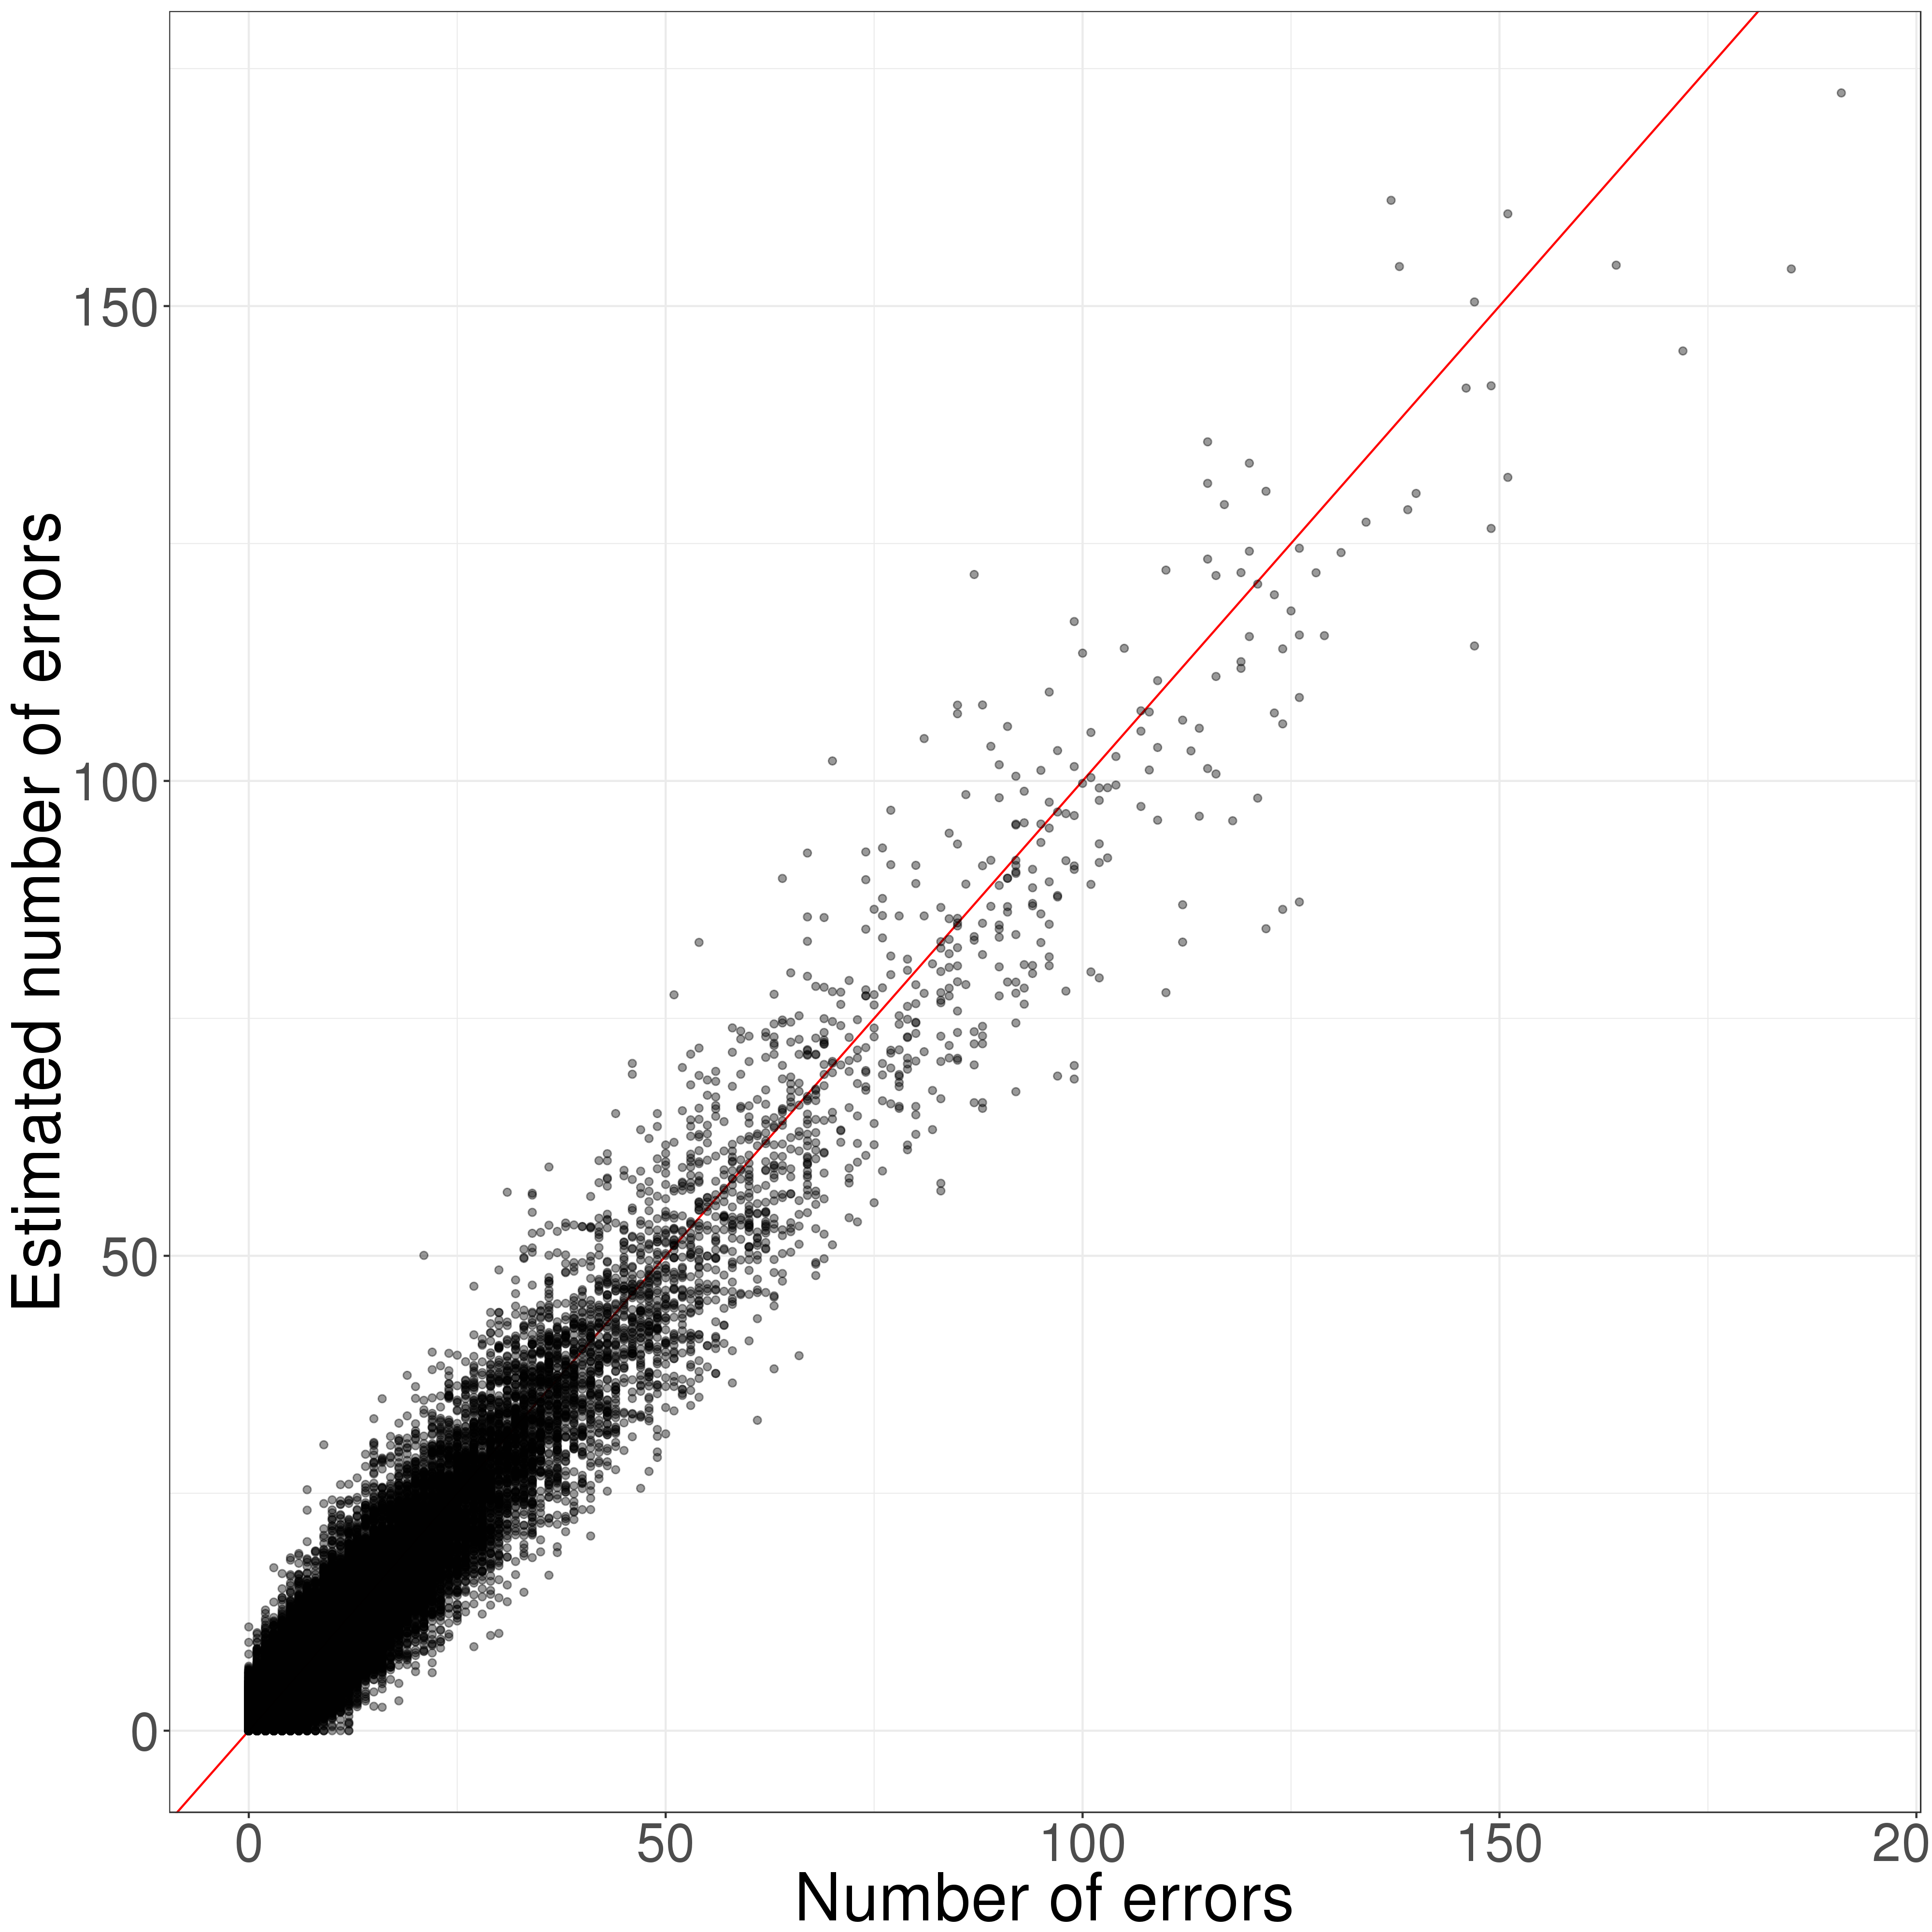
\includegraphics[width=\textwidth]{error-impute}}
\caption{Number of imputation errors vs the estimated number of imputation errors by SNP. For each SNP with missing data, the number of imputation errors corresponds to the number of individuals for which imputation is incorrect. The estimated number of errors is a quantity that is returned when imputing with snp\_fastimpute.}\label{fig:error-impute}
\end{figure}

\vspace{3em}

\begin{figure}[!h]
\centerline{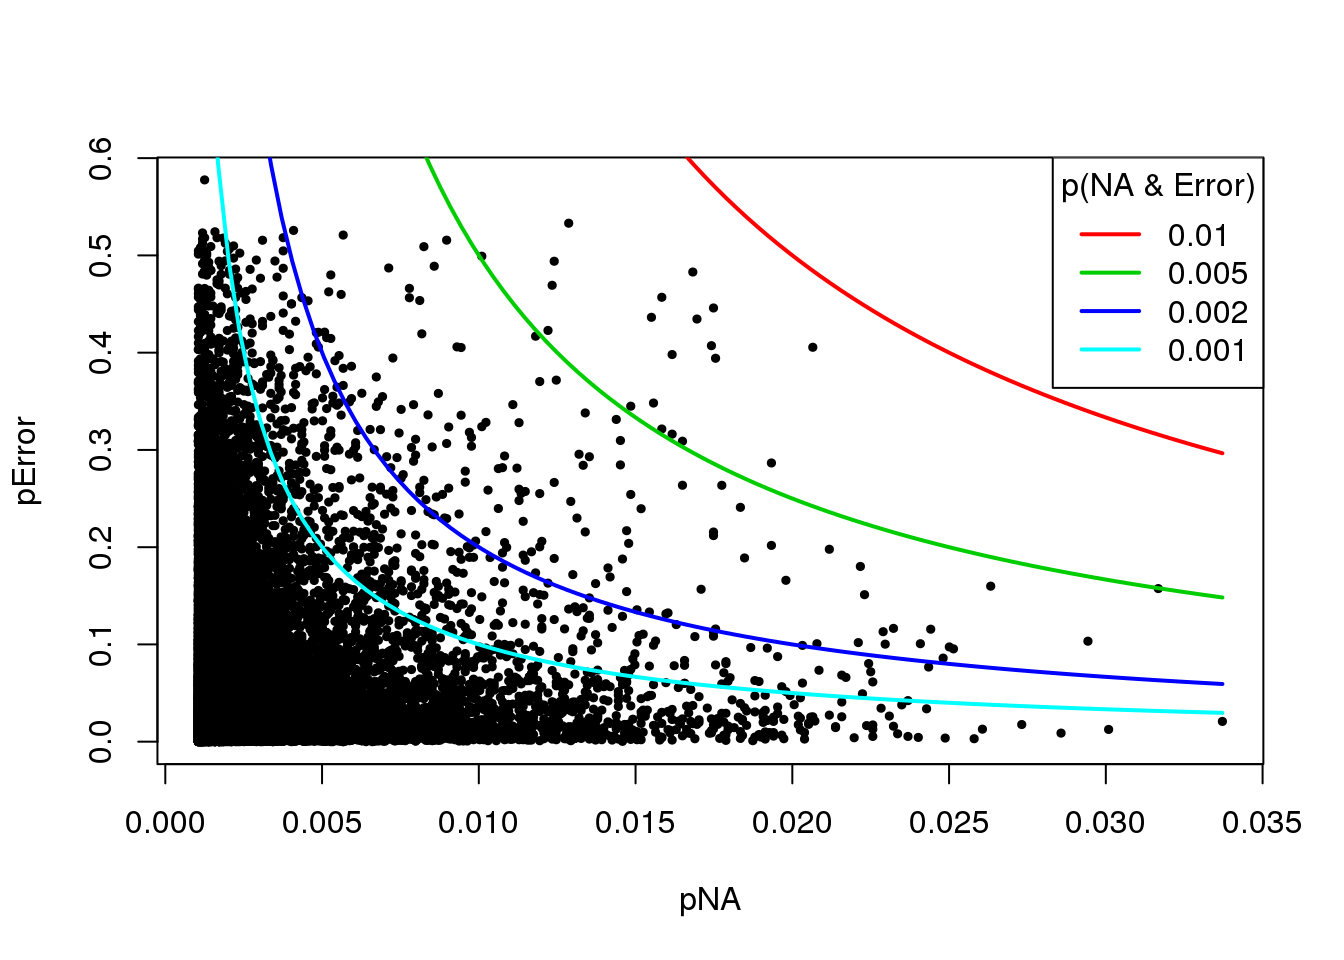
\includegraphics[width=\textwidth]{post-imputation}}
\caption{For each SNP (point), the estimated proportion of imputation errors ($\hat{p}(error~|~NA)$) vs the proportion of missing values ($p(NA) > 0.001$).
These results come from the imputation of the Celiac dataset with function snp\_fastImpute (Supplementary notebook ``preprocessing''). 
Colored curves are representing the estimated proportion of wrong genotypes per SNP ($\hat{p}(error~\&~NA) = \hat{p}(error~|~NA) \cdot p(NA)$). This particularly shows that no SNP has more than 1\% of wrong genotypes, allowing for no post-processing.}\label{fig:post-imputation}
\end{figure}

\clearpage
\subsection{Overview}

\begin{table}[!h]
\caption{Comparison of tools in low-level data management (first three rows) and high-level genetic analyses (the rest of rows). The bigstatsr and bigsnpr packages provide the most comprehensive and versatile infrastructure for data storage, processing and extensions; implement the main genetic analysis pipelines; and intrincically exploit memory-mapped files and parallel data processing.
Notes:
1: binary data format;
2: multi-core and cluster parallel computation;
3: support of imputed genotype data.
When comparing tools in terms of parallel computation, we do not consider the case of jobs manually distributed, e.g.\ splitting genotypes into batches. We are aware of the bitwise parallelism in PLINK 1.9, but this feature is used internally for specific computations; instead, we follow the official documentaion (https://www.cog-genomics.org/PLINK/1.9/parallel). The official documentation for the GenABEL project is at http://www.genabel.org/packages/ParallABEL.
GRM: Genetic Relationship Matrix; PCA: Principal Component Analysis; GWAS: Genome-Wide Association Study; PRS: Polygenic Risk Score.}
\begin{center}
\begin{adjustbox}{max width=\textwidth}
\begin{tabular}{|l|c|c|c|c|c|}
\hline
\multirow{2}{*}{Toolkit/Feature} & bigstatsr~/ & \multirow{2}{*}{PLINK 1.9} & \multirow{2}{*}{GCTA} & SNPRelate~/ & \multirow{2}{*}{GenABEL} \\
 & bigsnpr & & & GWASTools &  \\
\hline
\hline
Proper genotype data format & FBM$^{2,3}$ & ped/bed$^2$ & - & GDS$^{2,3}$ & databel$^{2,3}$ \\ \hline
Data format extension, e.g. -omics & $\checkmark$ & - & - & - & $\checkmark$ \\ \hline
Vector/Matrix operations & $\checkmark^1$ & - & - & - & $\checkmark^1$ \\ \hline
Quality Control & $\checkmark$ & $\checkmark$ & - & $\checkmark$ & $\checkmark$ \\ \hline
GRM & $\checkmark^1$ & $\checkmark^1$ & $\checkmark^1$ & $\checkmark^1$ & $\checkmark^1$ \\ \hline
PCA & $\checkmark^1$ & $\checkmark$ & $\checkmark^1$ & $\checkmark^1$ & - \\ \hline
GWAS & $\checkmark^1$ & $\checkmark$ & $\checkmark^1$ & $\checkmark$ & $\checkmark^1$ \\ \hline
PRS & $\checkmark$ & $\checkmark$ & - & - & - \\ \hline
\end{tabular}
\end{adjustbox}
\end{center}
\label{tab:andrey}
\end{table}


\end{document}
